

\chapter{Antecedentes}

\section{Estabilizaci\'{o}n de L\'{i}nea de Vista}
Un sistema de estabilizaci\'{o}n inercial, es un sistema que mantiene la l\'{i}nea de vista de un sensor electro\'{o}ptico cuando este est\'{a} sujeto a perturbaciones externas, bas\'{a}ndose en mediciones inerciales realimentadas a un sistema de control. La l\'{i}nea de vista es una l\'{i}nea recta imaginaria al largo de la cual un observador tiene una vista clara de un objetivo. Para definir la l\'{i}nea de vista de la carga \'{u}til\footnote{La carga \'{u}til o carga de pago es la capacidad de carga de un aeronave o un cohete de transporte, usualmente medido en t\'{e}rminos de peso. Dependiendo de la naturaleza de la misi\'{o}n de vuelo, la carga \'{u}til del veh\'{i}culo puede incluir carga, pasajeros, municiones, instrumentos cient\'{i}ficos u otro equipo.} de un UAV debemos primero tomar en cuenta que el campo de visi\'{o}n\footnote{Es la medida del mundo observable que se ve en cualquier momento dado. En el caso de instrumentos o sensores \'{o}pticos, es el \'{a}ngulo s\'{o}lido a trav\'{e}s del cual un detector es sensible a la radiaci\'{o}n electromagn\'{e}tica, abreviado FOV por sus siglas en ingl\'{e}s} de un sensor de imagen es menor a 360 grados, el centro de este campo de visi\'{o}n es la direcci\'{o}n de observaci\'{o}n y la l\'{i}nea con origen en el sensor y que se extiende a trav\'{e}s del centro del campo de visi\'{o}n hacia el infinito define la l\'{i}nea de vista del sensor de imagen abreviada como (LOS) por sus siglas en ingl\'{e}s, figura ~\ref{fig:LOSDef}. Para el alcance de esta tesis consideraremos que cualquier curvatura de la l\'{i}nea de vista entre el sensor y el objetivo, es peque\~{n}a y por lo tanto despreciable.

\begin{figure}[H]
\centering 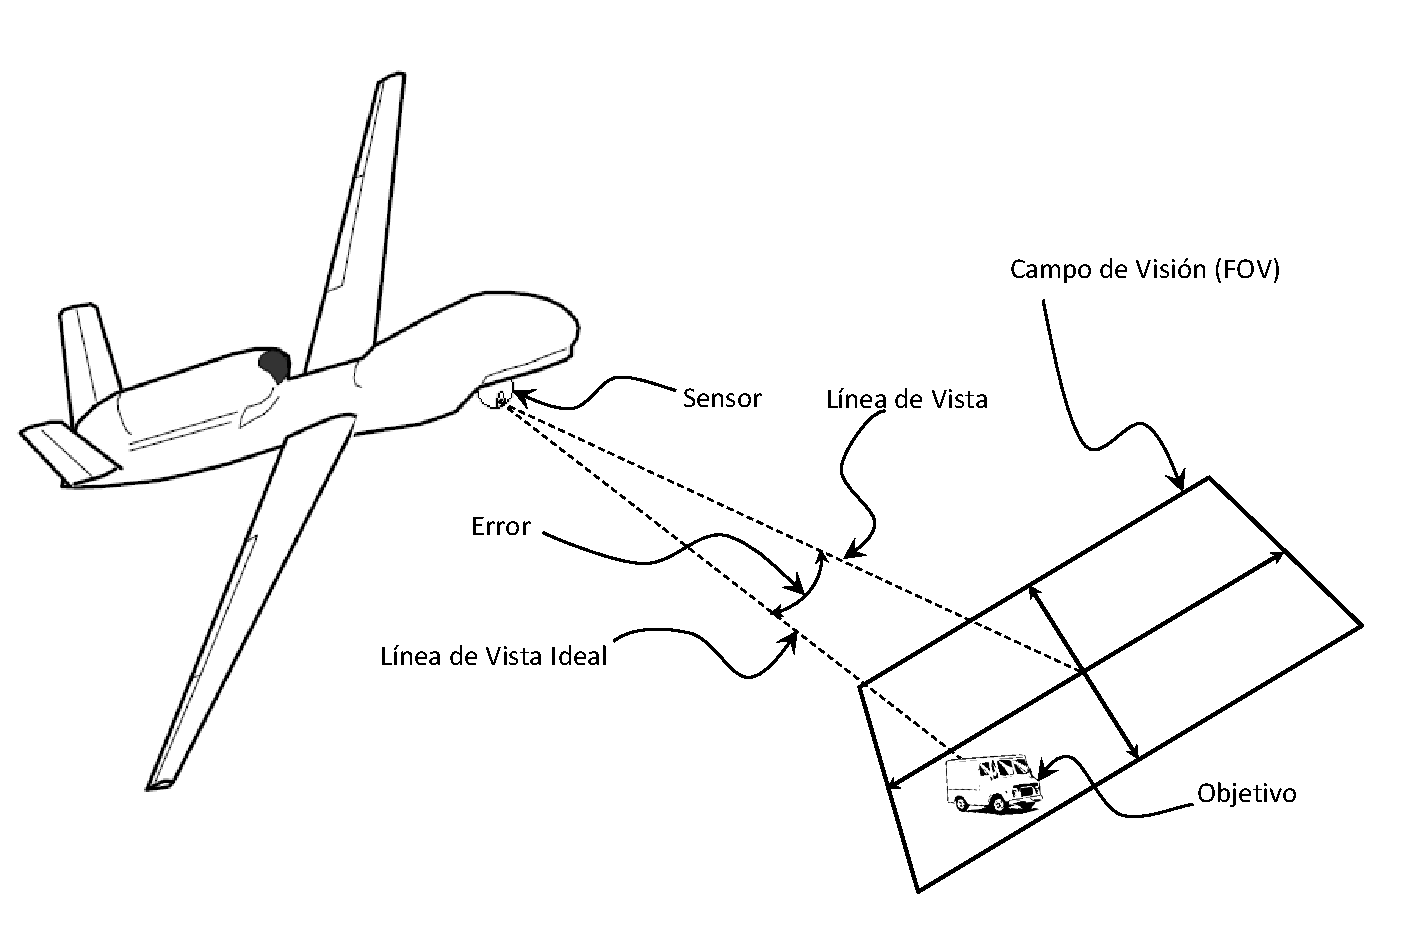
\includegraphics[scale=0.5]{img/LOSDef.pdf}
%trim = izquierda abajo derecha arriba
\caption{Definici\'{o}n de la L\'{i}nea de Vista}%Esta es la l\'{i}nea para el pie de figura
\label{fig:LOSDef}
\end{figure}

Entonces considerando lo mencionado anteriormente, podemos definir la estabilizaci\'{o}n de l\'{i}nea de vista como el acto de mantener el objetivo en el centro del campo de visi\'{o}n del sensor \'{o}ptico, bajo movimientos arbitrarios de la plataforma portadora del sistema y/o movimientos del objetivo a seguir. Se asume que la plataforma y el objetivo pueden moverse en los seis grados de libertad que definen la posici\'{o}n y orientaci\'{o}n de un cuerpo r\'{i}gido en el espacio tridimensional, que se definen por tres componentes de traslaci\'{o}n en tres ejes perpendiculares que describen los movimientos delante/atr\'{a}s, arriba/abajo e izquierda/derecha, combinados tres componentes de rotaci\'{o}n sobre los mismos tres ejes perpendiculares los cuales son com\'{u}nmente denominados en ingl\'{e}s como roll pitch y yaw, los cuales son conocidos como \'{a}ngulos n\'{a}uticos ya que son usados para describir la orientaci\'{o}n de una embarcaci\'{o}n o aeronave. Sin embargo el vector de la l\'{i}nea de vista tiene \'{u}nicamente dos grados de libertad debido a que la estabilizaci\'{o}n de l\'{i}nea de vista est\'{a} restringida al centro del campo de visi\'{o}n del sensor, en este contexto es posible que el objetivo se traslade y rote sobre el vector de la l\'{i}nea de vista y a\'{u}n as\'{i} satisfacer el prop\'{o}sito de estabilizaci\'{o}n. Un un sistema mec\'{a}nico capaz de mantener los dos \'{a}ngulos que definen el vector de l\'{i}nea de vista ideal es un sistema gimbal de dos ejes, el cual al rota el sensor alrededor de dos articulaciones angulares ortogonales que com\'{u}nmente consisten en un arreglo yaw/pitch.

Los dos marcos de referencia comunes para el mecanismo de estabilizaci\'{o}n son el marco inercial y el del campo de visi\'{o}n del sensor, estos se usan para medir el error entre la l\'{i}nea de vista medida y la deseada la cual centra el objetivo en el centro del campo de visi\'{o}n. La forma m\'{a}s com\'{u}n de estabilizaci\'{o}n de l\'{i}nea de vista consiste en medir las perturbaciones de la l\'{i}nea de vista en el marco inercial por medio de sensores inerciales. Esta informaci\'{o}n despu\'{e}s es usada en el sistema que controla los \'{a}ngulos de los eslabones del mecanismo de estabilizaci\'{o}n  para contrarrestar los movimientos del veh\'{i}culo y as\'{i} mantener fija l\'{i}nea de vista en el objetivo. Otro m\'{e}todo para estabilizar la l\'{i}nea de vista es medir la desviaci\'{o}n del objetivo del centro del campo de visi\'{o}n al procesar por medio de algoritmos de visi\'{o}n el v\'{i}deo obtenido por el sensor \'{o}ptico. Este m\'{e}todo es llamado "seguimiento de objetivo" y aunque en principio este m\'{e}todo parezca simple, en realidad tiene complicaciones importantes ya que se requiere un conocimiento preciso del campo de visi\'{o}n de la c\'{a}mara, una capacidad de procesamiento significativa para seguir el objetivo en tiempo real bajo variedad de condiciones de luz, y la trasformaci\'{o}n del error medido a las se\~{n}ales de control del sistema mec\'{a}nico \cite{26}. Este m\'{e}todo esta tambi\'{e}n sujeto a influencias externas tales como nubes que puedan obstruir el objetivo.

Los sistemas gimbal de estabilizaci\'{o}n de c\'{a}mara modernos combinan informaci\'{o}n obtenida de las mediciones de GPS, sensores inerciales, encoders, informaci\'{o}n de los estados del veh\'{i}culo e informaci\'{o}n de seguimiento de objetivo proveniente de una tarjeta de procesamiento de v\'{i}deo para generar una estabilizaci\'{o}n robusta.  
    



\section{Plataformas de Estabilizaci\'{o}n Inercial Aerotransportadas}

Las plataformas de estabilizaci\'{o}n inercial como se ha mencionado anteriormente, son usadas para estabilizar y apuntar un amplia variedad de sensores, c\'{a}maras, telescopios y sistemas de armas. Este tipo de sistemas se comenzaron a usarse desde hace aproximadamente cien a\~{n}os por lo que han sido usadas en todo tipo de veh\'{i}culos, desde sat\'{e}lites a submarinos e incluso en algunos dispositivos port\'{a}tiles \cite{29}. En especifico las plataformas de estabilizaci\'{o}n inercial aerotransportadas pueden ser de gran variedad de formas y tama\~{n}os las cuales generalmente est\'{a}n en funci\'{o}n del aeronave en la cual se montar\'{a}n para satisfacer un amplio rango de misiones y entre las cargas \'{u}tiles m\'{a}s comunes que se montan en una plataforma de estabilizaci\'{o}n inercial aerotransportada est\'{a}n:

\begin{itemize}
    \item Sistemas laser. (Tel\'{e}metros, Designadores)
    \item C\'{a}maras t\'{e}rmicas.
    \item C\'{a}maras electro \'{o}pticas de espectro visible.
    \item Antenas direccionales.   
\end{itemize}
La configuraci\'{o}n m\'{a}s com\'{u}n para un sistema gimbal de dos ejes es el llamado Pan-Tilt en el cual el primer eje, o el eje del eslab\'{o}n externo, permite la estabilizaci\'{o}n en el plano horizontal (paneo o acimut) mientras que el segundo eje, o el eje del eslab\'{o}n interno, permite la estabilizaci\'{o}n en el plano vertical (inclinaci\'{o}n o tilt). Las partes principales que componen un sistema de c\'{a}mara Pan-Tilt se muestran en la figura \ref{fig:CamParts}

\begin{figure}[H]
\centering 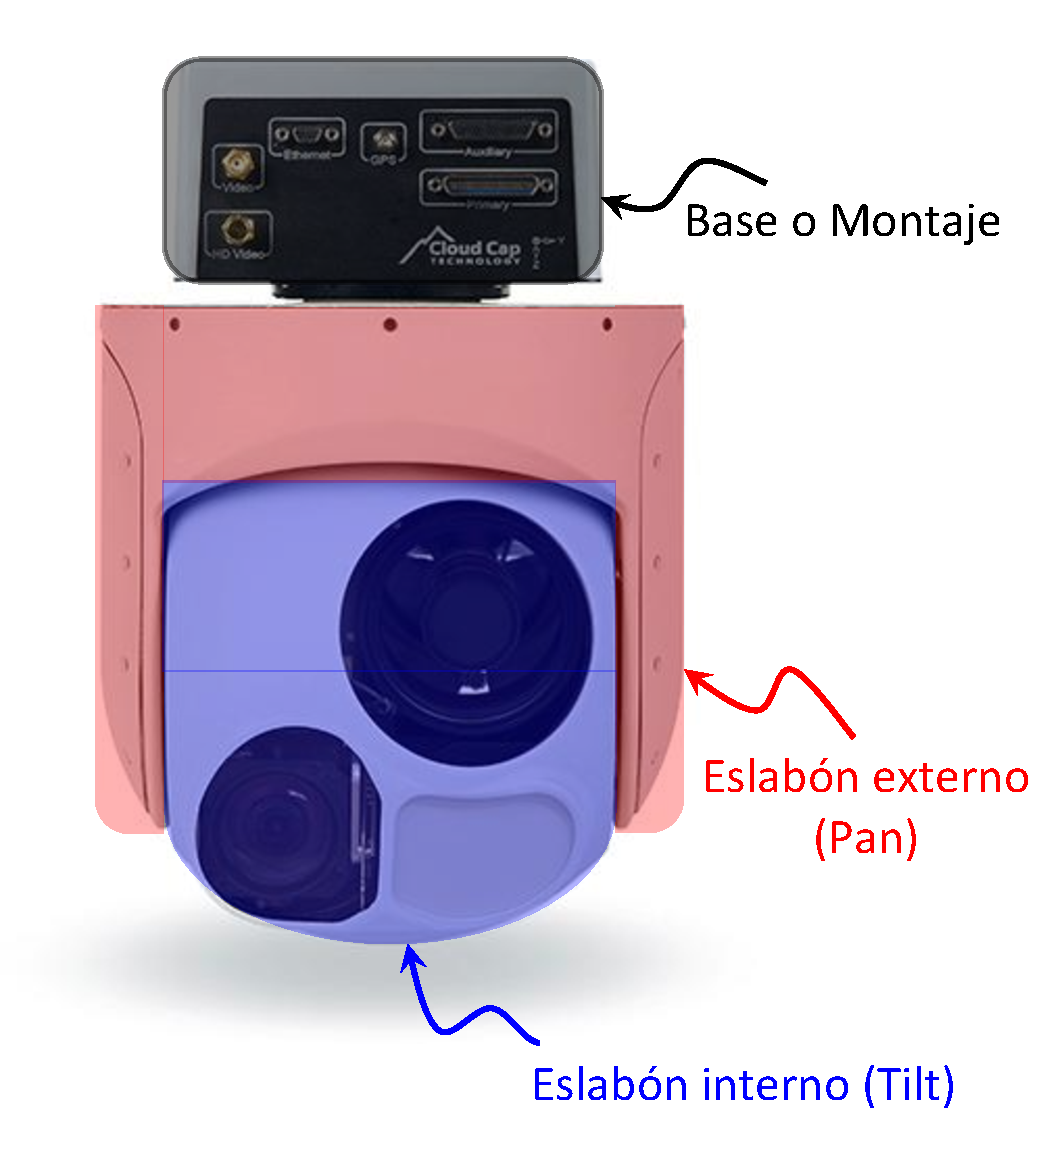
\includegraphics[scale=0.4]{img/GimbalParts.pdf}
%trim = izquierda abajo derecha arriba
\caption{Partes principales de un sistema de c\'{a}mara Pan-Tilt}%Esta es la l\'{i}nea para el pie de figura
\label{fig:CamParts}
\end{figure}

La base del gimbal es usualmente ligera y provee soporte estructural as\'{i} como aislamiento vibratorio al sistema gimbal mediante amortiguadores de vibraci\'{o}n de gel de silicio. El eslab\'{o}n externo provee a la c\'{a}mara de un movimiento de \textit{"paneo"} hacia la izquierda y derecha, el siguiente eslab\'{o}n, el interno lleva montada la carga \'{u}til y mueve la imagen de la c\'{a}mara hacia arriba y abajo (rotaci\'{o}n vertical) a \'{e}sta configuraci\'{o}n de gimbal se le conoce con diferentes nombres entre los cuales est\'{a}n: acimut/elevaci\'{o}n, pan/tilt o yaw/pitch La combinaci\'{o}n acimut/elevaci\'{o}n se refiere al horizonte terrestre y la combinaci\'{o}n yaw/pitch hace referencia a los \'{a}ngulos de n\'{a}uticos referenciados a un marco de referencia NED (Norte - Este - Abajo) por sus siglas en ingl\'{e}s. A lo largo de esta tesis usaremos la denominaci\'{o}n pan/tilt para referirnos a los \'{a}ngulos de los eslabones del gimbal.

Existe un amplio espectro de de sistemas gimbal, pero debido a que el uso de estos sistemas depende en gran medida de las capacidades de carga del aeronave que los transporta estos son clasificados principalmente en base a su peso total como: s\'{u}per ligeros, peque\~{n}os, medianos y grandes, en la figura ~\ref{fig:CamClases} se muestran ejemplos de sistemas gimbal ordenados seg\'{u}n su peso y tambi\'{e}n se muestra un ejemplo del tipo de aeronave capaz de llevar estos dispositivos, podemos concluir que un gimbal de mayor tama\~{n}o tendr\'{a} mayores capacidades de estabilizaci\'{o}n y m\'{a}s y mejores sensores, pero esto tambi\'{e}n incrementa las necesidades de un aeronave con mayor capacidad de carga.

\begin{figure}[h]
\centering 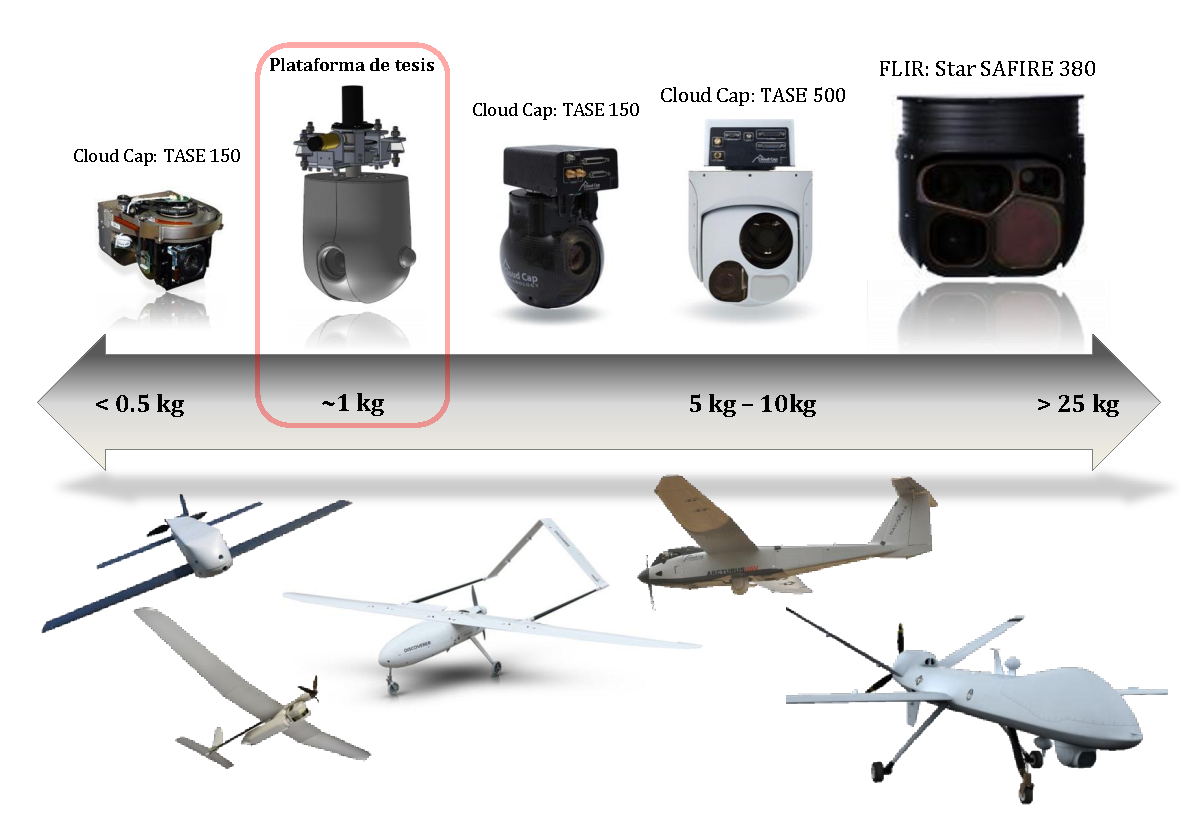
\includegraphics[scale=0.8]{img/Gimbalclases1.pdf}
%trim = izquierda abajo derecha arriba
\caption{Clasificaci\'{o}n de gimbals aerotransportados}%Esta es la l\'{i}nea para el pie de figura
\label{fig:CamClases}
\end{figure}

Los gimbals s\'{u}per ligeros, son aquellos qe tienen un peso de 0.5 kg o menos y son usado t\'{i}picamente por los vant's lanzados manualmente con un peso bruto de despegue m\'{a}ximo de alrededor de 2 a 5 kg. Estos gimbals pueden estabilizar una carga \'{u}til de hasta dos c\'{a}maras con dispositivo de carga acoplada (CCD) o una sola c\'{a}mara de bloque con zoom variable. Este tipo de gimbals son dise\~{n}ados espec\'{i}ficamente para la plataforma en la que ser\'{a}n utilizados y es necesario considerar que su forma afectar\'{a} su aerodin\'{a}mica, pues el sistema gimbal representar\'{a} una parte significativa de la superficie total del aeronave. la precisi\'{o}n en la estabilizaci\'{o}n de linea de vista alcanzada por estos dispositivos es t\'{i}picamente de $\pm0.5$ grados.

Los gimbals peque\~{n}os est\'{a}n en un rango de peso de entre los 0.5 y 5 kg. estos gimbals siguen teniendo limitaciones en su peso y forma, pero estos tienen una forma m\'{a}s cil\'{i}ndrica que permite el rango de movimiento completo que se aprecia en sistemas de mayor tama\~{n}o. Los gimbals de esta clase pueden com\'{u}nmente llevar dos tipos de cargas \'{u}tiles ofreciendo combinaciones interesantes en la resoluci\'{o}n del la c\'{a}mara y distancias focales. El error t\'{i}pico de los gimbals peque\~{n}os esta entre los $\pm0.5$ y los $\pm0.1$ grados.

Los sistemas de la clase media y grande, cuyos pesos van de los 5 a los 10 kg y mayores a los 25 kg respectivamente tienen una gran capacidad de combinaci\'{o}n de m\'{u}ltiples sensores. Estos sistemas son utilizados en veh\'{i}culos de gran autonom\'{i}a con intervalos de 8 a 24 horas y necesitan proveer al operador de un amplia variedad de opciones de captura de v\'{i}deo para manejar los cambios en las condiciones de luz que se presenten durante la duraci\'{o}n del vuelo. Estos gimbals tienen un error menor a los $\pm0.1$ grados pero est\'{a}n sometidos a una mayor exigencia debido la gran altitud que deben alcanzar las aeronaves que usan esta clase de sistemas ya que estas poseen grandes firmas ac\'{u}sticas\footnote{El t\'{e}rmino firma ac\'{u}stica es usado para describir las emisiones ac\'{u}sticas generadas por un aeronave y es de vital importancia para en aquellas aeronaves destinadas a misiones de vigilancia pues de este par\'{a}metro depende la altitud que ser\'{a} necesaria alcanzar para no ser detectado por el objetivo}.

\section{Integraci\'{o}n de los Sistemas de Estabilizaci\'{o}n Inercial}

En la integraci\'{o}n de un sistema gimbal en un aeronave no tripulada existen algunas cuestiones importantes que tienen que ser consideradas. Los veh\'{i}culos a\'{e}reos no tripulados se basan en un enlace de comunicaciones que envia comandos de mando y control al sistema gimbal. Debido a la latencia\footnote{En redes inform\'{a}ticas de datos se denomina latencia a la suma de retardos temporales dentro de una red. Un retardo es producido por la demora en la propagaci\'{o}n y transmisi\'{o}n de paquetes de datos dentro de la red.} y la calidad del enlace, los comandos pueden sufrir un retardo significativo desde el momento en el que el operador env\'{i}a los comandos y el sistema gimbal los recibe. 

\begin{figure}[H]
\centering 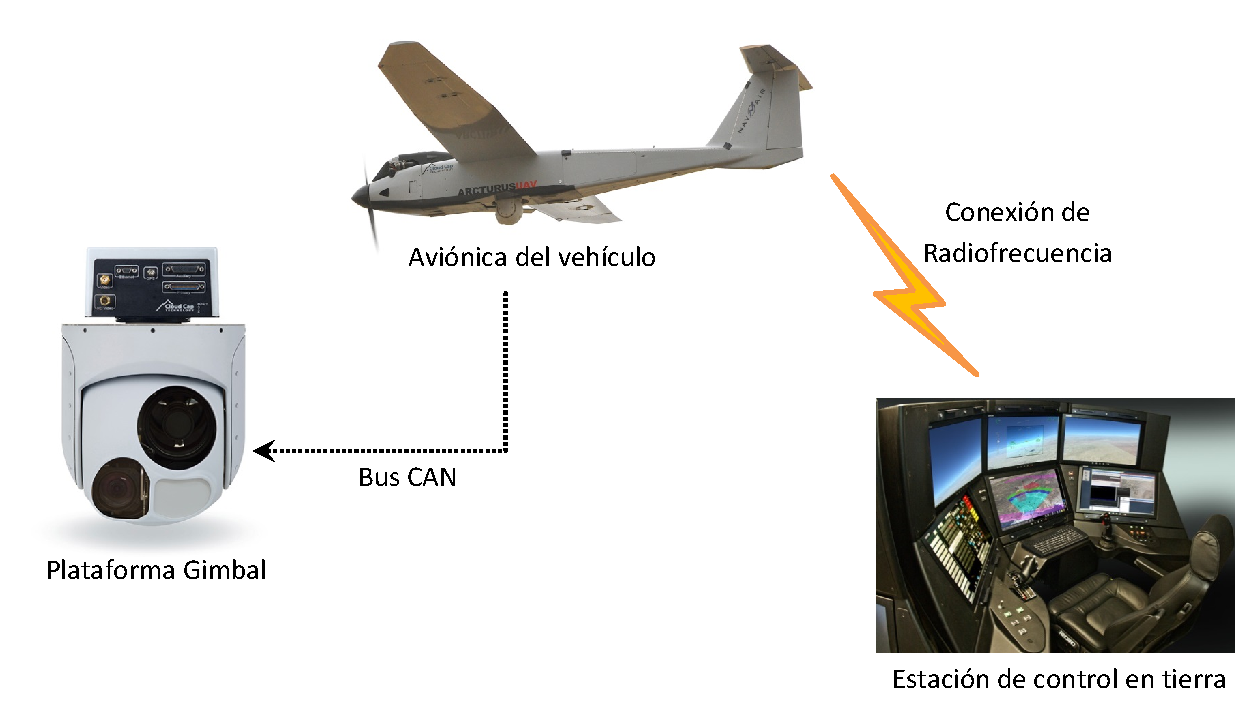
\includegraphics[scale=0.5]{img/integration.pdf}
%trim = izquierda abajo derecha arriba
\caption{Ejemplo de enlace de integraci\'{o}n gimbal-VANT}%Esta es la l\'{i}nea para el pie de figura
\label{fig:Integration}
\end{figure}

Estos retardos pueden dificultarle a un operador el seguimiento de un objetivo usando \'{u}nicamente un control manual, es por esto que caracter\'{i}sticas tales como se\~{n}alamiento a un punto GPS, seguimiento de trayectoria, e incluso triangulaci\'{o}n se integran a bordo del sistema gimbal y es com\'{u}n encontrar estas caracter\'{i}sticas en plataformas de gran tama\~{n}o, sin embargo, recientemente estas caracter\'{i}sticas comienzan a aparecer en sistemas m\'{a}s peque\~{n}os gracias al incremento de poder de procesamiento de los sistemas electr\'{o}nicos.

Los sistemas a\'{e}reos no tripulados (SANTs) deben proveer una conexi\'{o}n de datos bidirecional entre el operador y el gimbal para comando y control as\'{i} como para monitorear su estado. En los sistemas comerciales existe una tendencia a usar un protocolo CAN\footnote{CAN (acr\'{o}nimo del ingl\'{e}s Controller Area Network) es un protocolo de comunicaciones desarrollado por la firma alemana Robert Bosch GmbH, basado en una topolog\'{i}a bus para la transmisi\'{o}n de mensajes en entornos distribuidos} para la comunicaci\'{o}n entre el sistema de estabilizaci\'{o}n y la avi\'{o}nica del veh\'{i}culo. Los SANTs deben tambi\'{e}n proveer una conexi\'{o}n de datos que pueda transmitir el v\'{i}deo obtenido en tiempo real al operador. Se ha determinado por medio de pruebas, que una latencia mayor de 100-250ms entre el env\'{i}o del comando y la respuesta mostrada en el v\'{i}deo reduce significativamente la efectividad del operador durante el control manual del sistema, existen varias maneras de reducir este problema, una de las cuales es mejorar la conexi\'{o}n de datos al usar transmisores y receptores de mayor potencia para reducir la latencia, sin embargo esto no siempre es posible adem\'{a}s de la existencia de l\'{i}mites intr\'{i}nsecos en los sistemas de telecomunicaciones, otro enfoque consiste en aumentar la autonom\'{i}a del gimbal al embarcar algoritmos de se\~{n}alamiento por coordenadas GPS o algoritmos seguimiento basados en visi\'{o}n, de tal manera que se incremente la m\'{a}xima latencia permitida al dotar al sistema gimbal de la capacidad de realizar tareas de forma aut\'{o}noma durante la espera de la recepci\'{o}n de un nuevo comando de control de parte del operador lo que provee una estabilizaci\'{o}n a largo plazo mucho m\'{a}s all\'{a} de \'{u}nicamente la estabilizaci\'{o}n inercial bajo control manual. 

Otro factor clave en la integraci\'{o}n del sistema gimbal es el entorno vibratorio al cual estar\'{a} expuesto. Las aeronaves que poseen la capacidad de carga \'{u}til en volumen y peso necesarias para llevar gimbals de clase media son com\'{u}nmente propulsados por motores de combisti\'{o}n interna de 2 a 4 tiempos los cuales producen grandes pulsos de par debido a la naturaleza no continua de su operaci\'{o}n. Estos pulsos de par est\'{a}n com\'{u}nmente en el rango de los 50-80Hz y sin un aislamiento vibratorio espec\'{i}fico, puede causar desenfoque en la imagen y fluctuaciones en el sistema de control. La propulsi\'{o}n de tipo el\'{e}ctrica proporciona un sistema de par continuo, por lo que su comportamiento vibratorio es de una frecuencia mucho mayor a los motores de combusti\'{o}n interna, este tipo de vibraciones son m\'{a}s f\'{a}ciles de amortiguar y tienen un menor efecto en la calidad de la imagen. Sin embargo estas est\'{a}n limitadas a llevar \'{u}nicamente cargas \'{u}tiles peque\~{n}as debido a las limitaciones energ\'{e}ticas de sus bater\'{i}as. Las aeronaves con propulsi\'{o}n el\'{e}ctrica tienen una ventaja adicional pues tienen una firma ac\'{u}stica significativamente menor, lo que permite al veh\'{i}culo volar m\'{a}s cerca del objetivo y con esto reducir los requerimientos de estabilizaci\'{o}n del sistema gimbal y en consecuencia tambi\'{e}n su tama\~{n}o .

\section{Entorno Operativo}

El sistema desarrollado en este trabajo esta dise\~{n}ado para operar en Veh\'{i}culos No Tripulados peque\~{n}os con una capacidad de carga de aproximadamente 1.5 kg. Las altitudes de crucero t\'{i}picas para estos veh\'{i}culos est\'{a}n entre los 150 a los 600 metros sobre nivel de suelo y con una velocidad de viento en calma de 50 a 110 km/h. Si bien esto representa una peque\~{n}a secci\'{o}n del espacio a\'{e}reo, esta es tambi\'{e}n una secci\'{o}n particularmente susceptible a turbulencias impredecibles. En este rango las corrientes de aire son afectadas por la geograf\'{i}a, construcciones humanas, calentamiento de la superficie terrestre, adicionalmente a las condiciones clim\'{a}ticas. 

Lo anterior implica que un veh\'{i}culo peque\~{n}o es m\'{a}s susceptible a las turbulencias lo cual eleva las exigencias de estabilizaci\'{o}n. La baja inercia, carga alar y masa reducida a\~{n}ade vulnerabilidad a las turbulencias a los VANTs peque\~{n}os. En \cite{26} se obtienen datos de emp\'{i}ricos a partir de pruebas de vuelo en un VANT peque\~{n}o con un autopiloto trabajando a una frecuencia de 10Hz. En los resultados de estas pruebas se observa que aproximadamente el 99\% del tiempo de vuelo, la velocidad angular de veh\'{i}culo es de 2 rad/seg o menor. Estos datos son \'{u}tiles al elegir las perturbaciones a las que expone el modelo para el dise\~{n}o del algoritmo de control en las simulaci\'{o}nes desarrolladas en el cap\'{i}tulo ~\ref{sec:ControlChapter}. 

\section{Revisi\'{o}n Bibliogr\'{a}fica} 

En esta tesis se estudia la configuraci\'{o}n de un gimbal de dos ejes Pan-Tilt as\'{i} como un m\'{e}todo para la estabilizaci\'{o}n de la l\'{i}nea de vista, este tema ya ha sido discutido y analizado en muchos estudios previos bajo diferentes consideraciones y m\'{e}todos. En \cite{8}, \cite{9}, A.K. Rue realiza algunos de los primeros trabajos de investigaci\'{o}n sobre el tema siendo de las referencias m\'{a}s antiguas, en estos trabajos se obtiene y estudia la din\'{a}mica y el acoplamiento geom\'{e}trico de un mecanismo gimbal de dos ejes para el caso simplificado en el que los elementos del gimbal est\'{a}n balanceados y suspendidos sobre los ejes principales de inercia.  


En \cite{3}, Peter J. Kennedy desarrolla el modelo de un sistema gimbal de dos ejes, bajo la hip\'{o}tesis que cada eslab\'{o}n esta balanceado y que los ejes de rotaci\'{o}n est\'{a}n alineados con los ejes principales de inercia, tambi\'{e}n se estudian a fondo dos arquitecturas de control de estabilizaci\'{o}n, la directa y la indirecta, concluyendo que el enfoque directo es el que mejor desempe\~{n}o tiene. En \cite{4}, Ekstrand desarrolla el modelo del gimbal de dos grados de libertad empleando las ecuaciones de cuerpos r\'{i}gidos de Euler as\'{i} como el m\'{e}todo de Lagrange y demostr\'{o} que la mayor\'{i}a de las perturbaciones inerciales pueden ser eliminadas bajo ciertas condiciones de simetr\'{i}a. En \cite{5}, M. Abdo, desarroll\'{o} las ecuaciones de movimiento para el caso en el que existen masas no balanceadas en el sistema, es decir las matrices de inercia no son diagonales, esto con el objetivo de estudiar los efectos del acoplamiento cruzado, adem\'{a}s en \cite{6} dise\~{n}a un lazo de control PID en cascada para el control del sistema y prueba por medio de simulaci\'{o}n el desempe\~{n}o del algoritmo de control dise\~{n}ado. En \cite{10} se estudia el efecto de las perturbaciones no lineales debidas a la fricci\'{o}n y proponen un algoritmo LQR basado en una ecuaci\'{o}n diferencial linear de primer orden para estimar y compensar tales perturbaciones obteniendo un desempe\~{n}o considerablemente superior a un PI convencional. En \cite{11} se aborda el problema de la presencia de    incertidumbres en los par\'{a}metros de la fricci\'{o}n del motor desarrollando un m\'{e}todo para mejorar la convergencia del sistema basado en control \'{o}ptimo.

En la literatura, se han desarrollado y dise\~{n}ado sistemas de control para los sistemas gimbal de dos grados de libertad aplicando diferentes m\'{e}todos de control incluyendo el tratado a fondo en esta tesis, es decir el control por modos deslizantes. En \cite{12} se presenta una propuesta de control por modos deslizantes basado en un observador PI, mientras que en \cite{13} se desarrolla un control por modos deslizantes bajo la consideraci\'{o}n de canales id\'{e}nticos de elevaci\'{o}n y paneo. En \cite{14}, se propone un control por modos deslizantes \textit{"Proxy-based"} el cual es un un control por modos deslizantes adaptado al entorno discreto introducido por Kikuuwe y Fujimoto en el 2006 para control de robots. Adem\'{a}s de las t\'{e}cnicas de control convencionales tambi\'{e}n se han realizado investigaciones aplicando algunas t\'{e}cnicas avanzadas entre las cuales podemos mencionar al control adaptable por redes neuronales desarrollado en \cite{15}, al control robusto por din\'{a}mica inversa \cite{16}, Control por l\'{o}gica difusa en \cite{17} y a la metodolog\'{i}a de control robusto H$\infty$ \cite{18}, sin embrago la mayor\'{i}a de estas t\'{e}cnicas avanzadas son complejas y dif\'{i}ciles de implementar. 